% Error distribution chart
\begin{figure}[htbp]
\centering
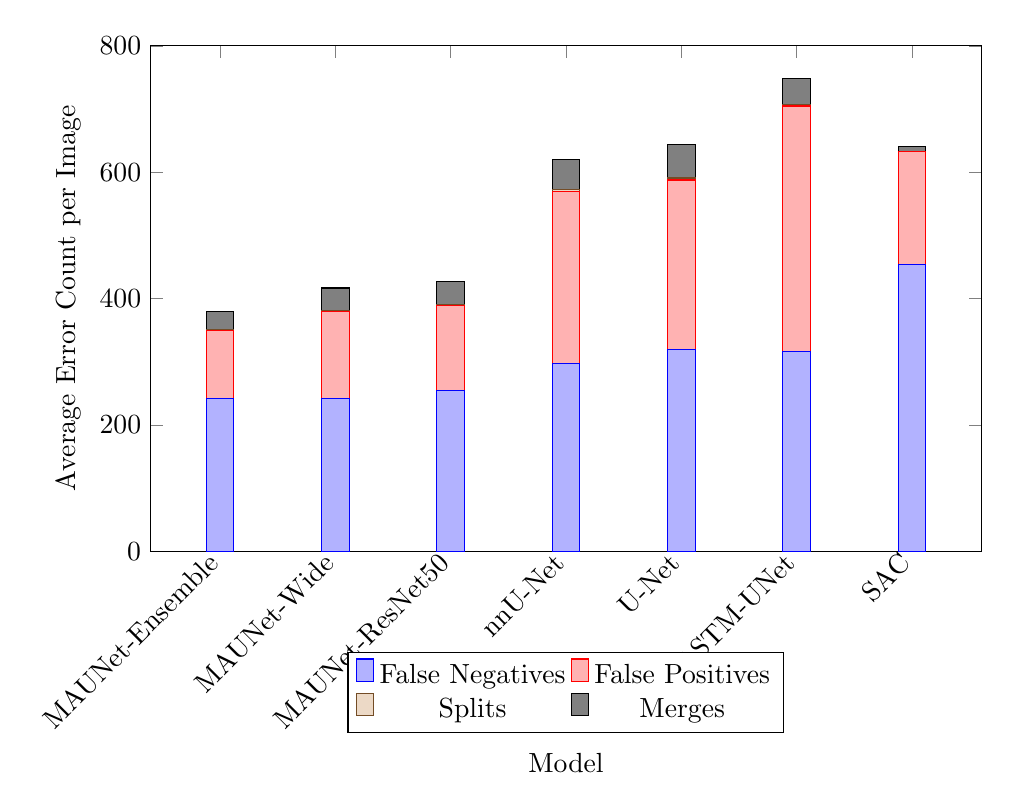
\begin{tikzpicture}
\begin{axis}[
    ybar stacked,
    width=\textwidth,
    height=8cm,
    xlabel={Model},
    ylabel={Average Error Count per Image},
    symbolic x coords={MAUNet-Ensemble, MAUNet-Wide, MAUNet-ResNet50, nnU-Net, U-Net, LSTM-UNet, SAC},
    xtick=data,
    x tick label style={rotate=45, anchor=east},
    legend style={at={(0.5,-0.2)}, anchor=north, legend columns=2},
    ymin=0,
    ymax=800
]

% False Negatives (bottom layer)
\addplot coordinates {
    (MAUNet-Ensemble, 241.0)
    (MAUNet-Wide, 241.0)
    (MAUNet-ResNet50, 254.7)
    (nnU-Net, 296.4)
    (U-Net, 319.6)
    (LSTM-UNet, 315.8)
    (SAC, 453.5)
};

% False Positives
\addplot coordinates {
    (MAUNet-Ensemble, 109.0)
    (MAUNet-Wide, 139.1)
    (MAUNet-ResNet50, 134.6)
    (nnU-Net, 272.7)
    (U-Net, 268.0)
    (LSTM-UNet, 389.0)
    (SAC, 179.0)
};

% Splits
\addplot coordinates {
    (MAUNet-Ensemble, 1.3)
    (MAUNet-Wide, 1.3)
    (MAUNet-ResNet50, 0.9)
    (nnU-Net, 3.6)
    (U-Net, 3.1)
    (LSTM-UNet, 1.7)
    (SAC, 0.1)
};

% Merges
\addplot coordinates {
    (MAUNet-Ensemble, 28.3)
    (MAUNet-Wide, 35.2)
    (MAUNet-ResNet50, 36.9)
    (nnU-Net, 47.3)
    (U-Net, 53.1)
    (LSTM-UNet, 41.8)
    (SAC, 8.2)
};

\legend{False Negatives, False Positives, Splits, Merges}
\end{axis}
\end{tikzpicture}
\caption{Error Type Distribution Across Models}
\label{fig:error_distribution}
\begin{quote}
\small
Stacked bar chart showing the distribution of different error types across all evaluated models. Models are ordered by total error count (lowest to highest). Key observations: (1) False negatives dominate error patterns across all models, (2) MAUNet variants show significantly lower total errors, (3) LSTM-UNet suffers from high false positive rates, (4) Split and merge errors are relatively rare across all architectures. This visualization guides optimization efforts by highlighting the primary error sources for each model architecture.
\end{quote}
\end{figure}
